\chapter{Phân tích thiết kế hệ thống}
\section{Tổng quan các chức năng}
\subsection{Biểu đồ use case tổng quan}
\begin{figure}[H]
    \centering
    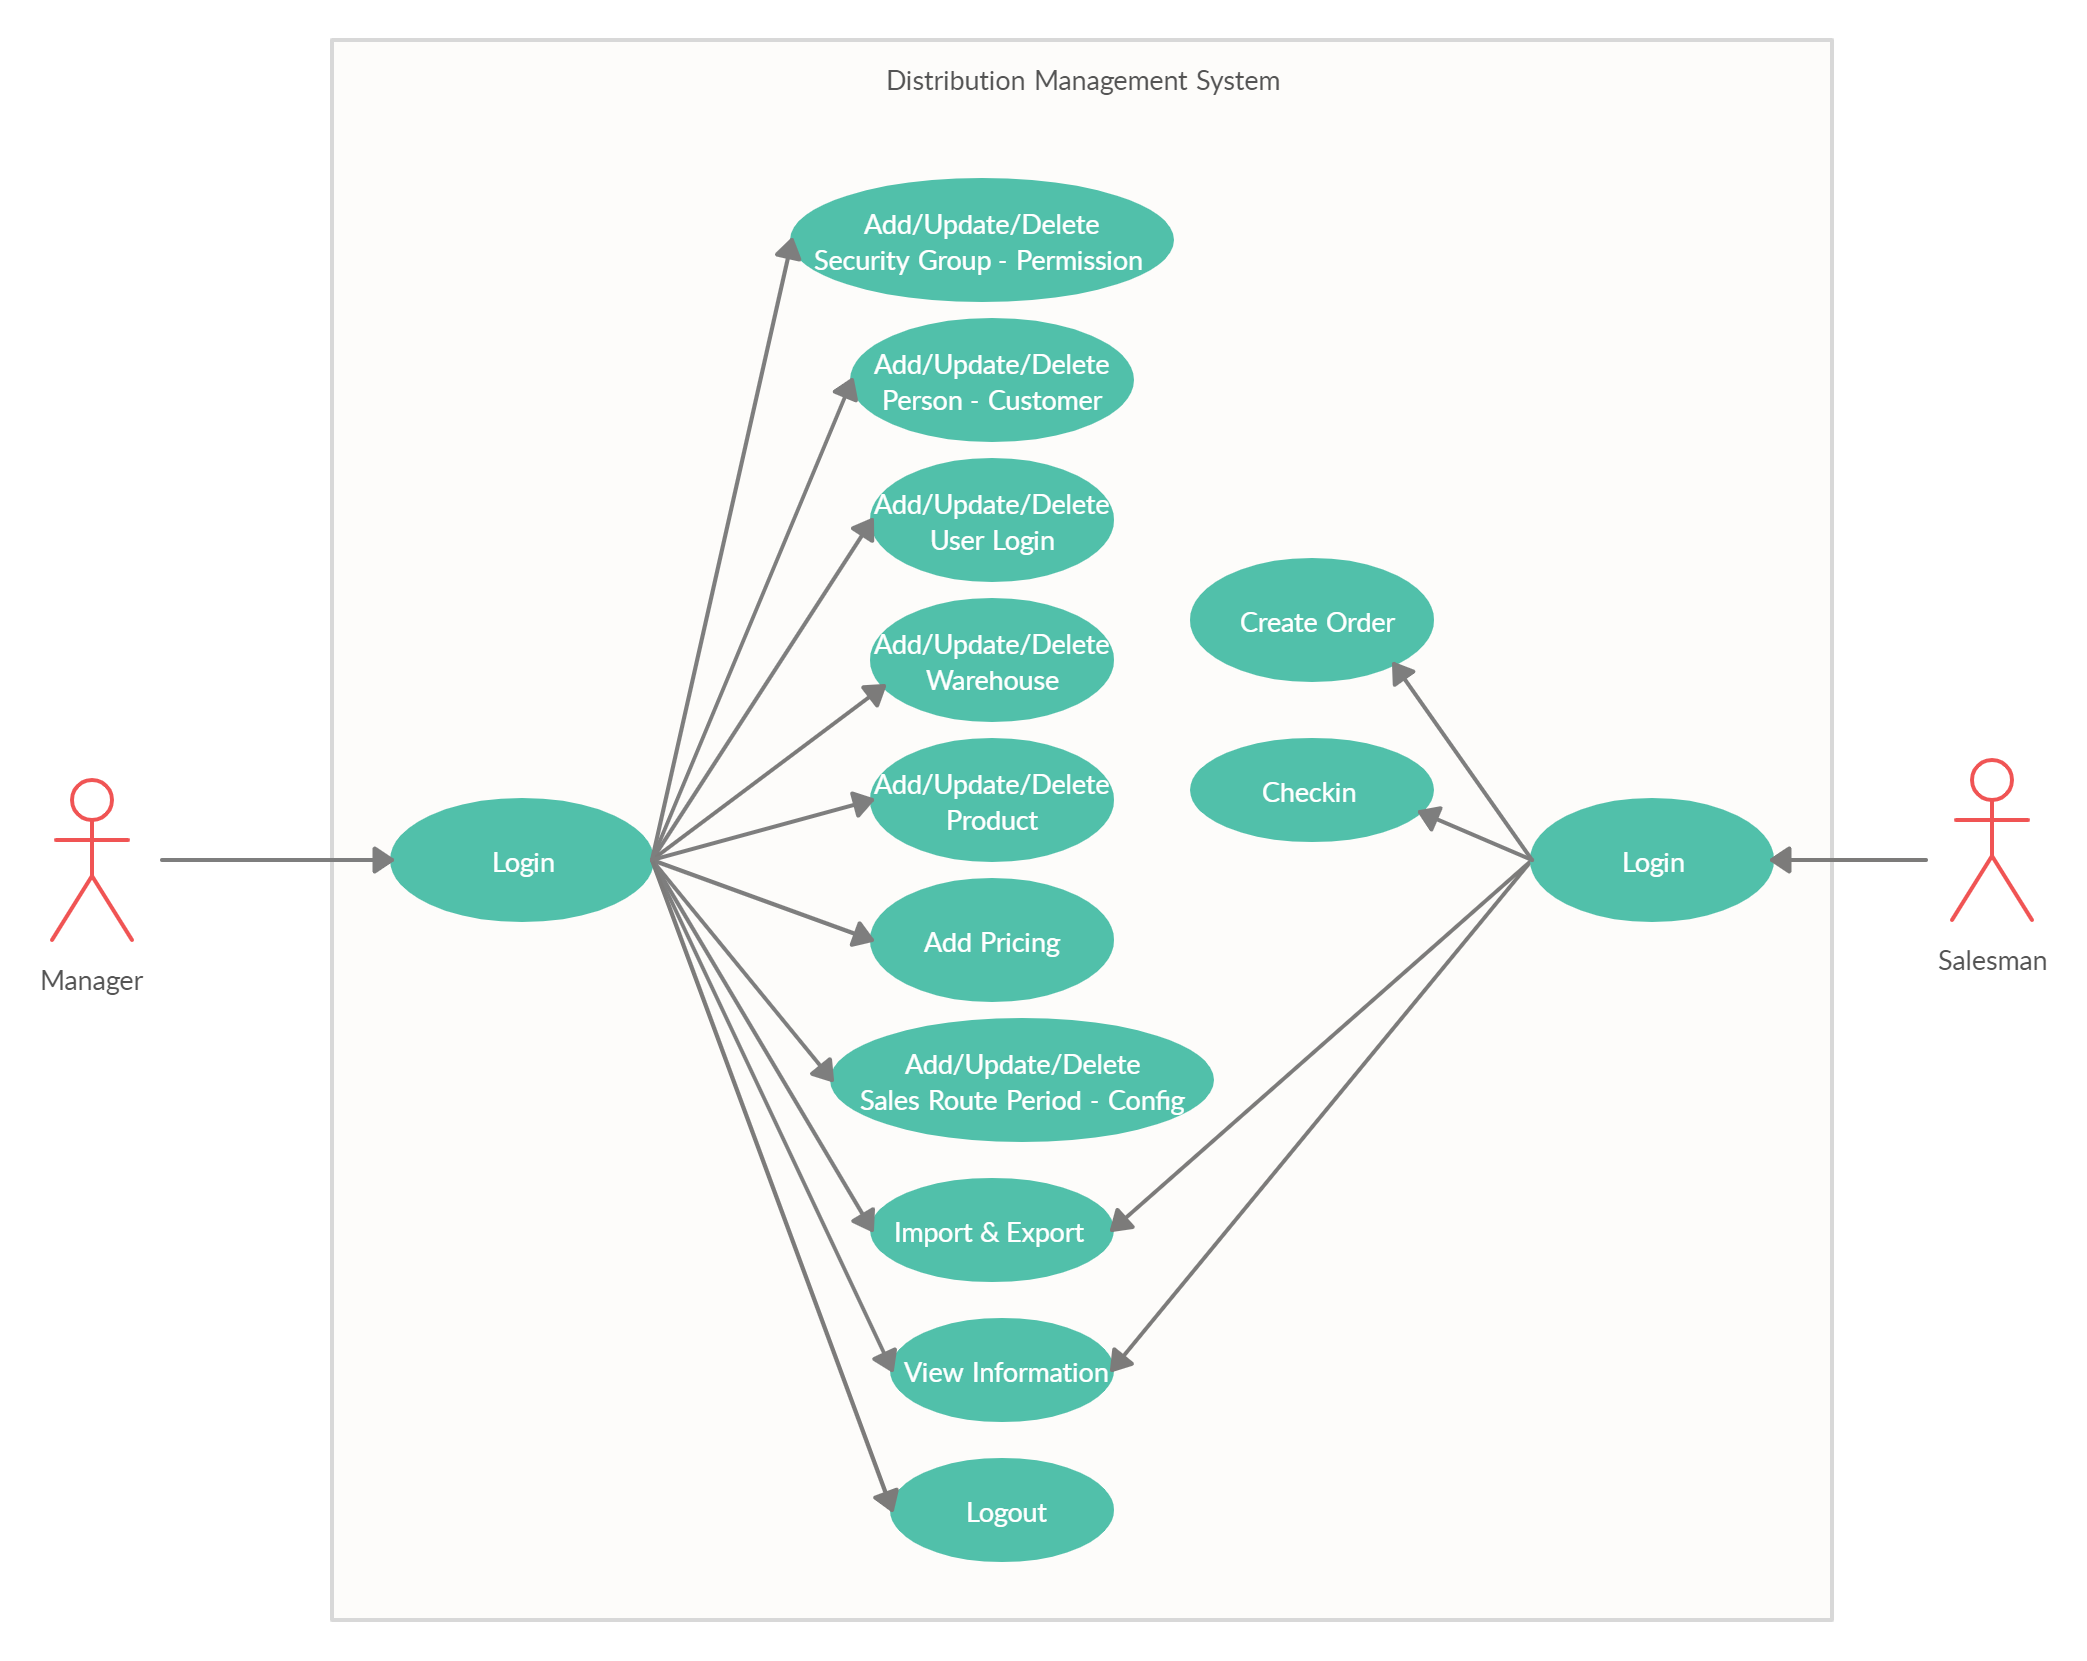
\includegraphics[width=12cm]{images/use-case/use-case-summary.jpg}
    \caption{Biểu đồ use case tổng quan}
\end{figure}

Hai tác nhân chính trong biểu đồ use case tổng quan
là người quản lý (manager) và nhân viên bán hàng (salesman).
Người quản lý ở đây là từ dùng chung, đại diện cho những người
quản lý nghiệp vụ riêng (quản lý sản phẩm, quản lý hàng tồn kho,
quản lý kho, quản lý giao dịch, quản lý tuyến bán hàng).
Người quản lý sau khi đăng nhập vào hệ thống có thể thực hiện
các nghiệp vụ quản lý như thêm / sửa / xóa sản phẩm, người dùng, …
Nhân viên bán hàng sau khi đăng nhập có thể xem được lịch
trình di chuyển của mình, lên hóa đơn mua hàng, check-in.

\subsection{Biểu đồ use case phân rã các chức năng của hệ thống}
Trong phần này, em sẽ trình bày các ca sử dụng chính trong hệ
thống, đưa ra biểu đồ use case và biểu đồ hoạt động chỉ cách
thức tương tác của người dùng với giao diện hệ thống. Do nhiều thao
tác có tính chất tương đồng nên em sẽ đưa ra các biểu
đồ hoạt động điển hình, các thao tác khác được thực hiện tương tự.

\subsubsection{Quản lý người dùng và phân quyền}
Biểu đồ use case cho ca sử dụng quản lý người dùng

\begin{figure}[H]
\centering
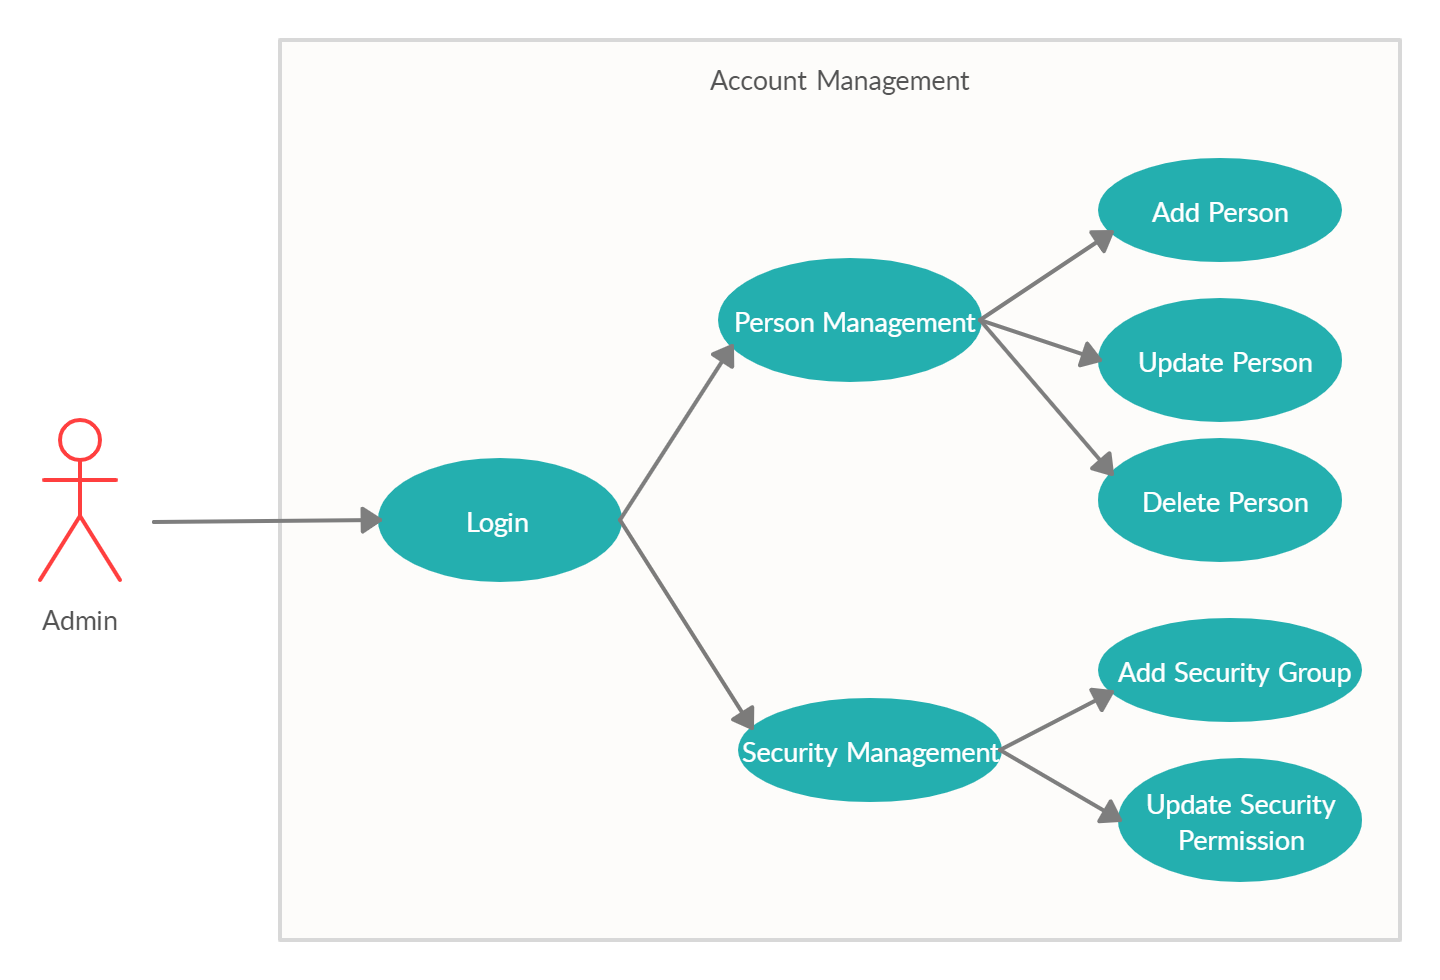
\includegraphics[width=12cm]{images/use-case/account-management.jpg}
\caption{Use-case quản lý người dùng}
\end{figure}

Người quản trị (admin) có thể quản lý các người dùng trong
hệ thống, quản lý quyền hạn của người dùng. Có thể thêm / sửa /
xóa người dùng, khách hàng, thêm / sửa quyền cho các người
quản lý cấp dưới.


Biểu đồ hoạt động cho các thao tác trong quản lý người dùng:
\begin{figure}[H]
\centering
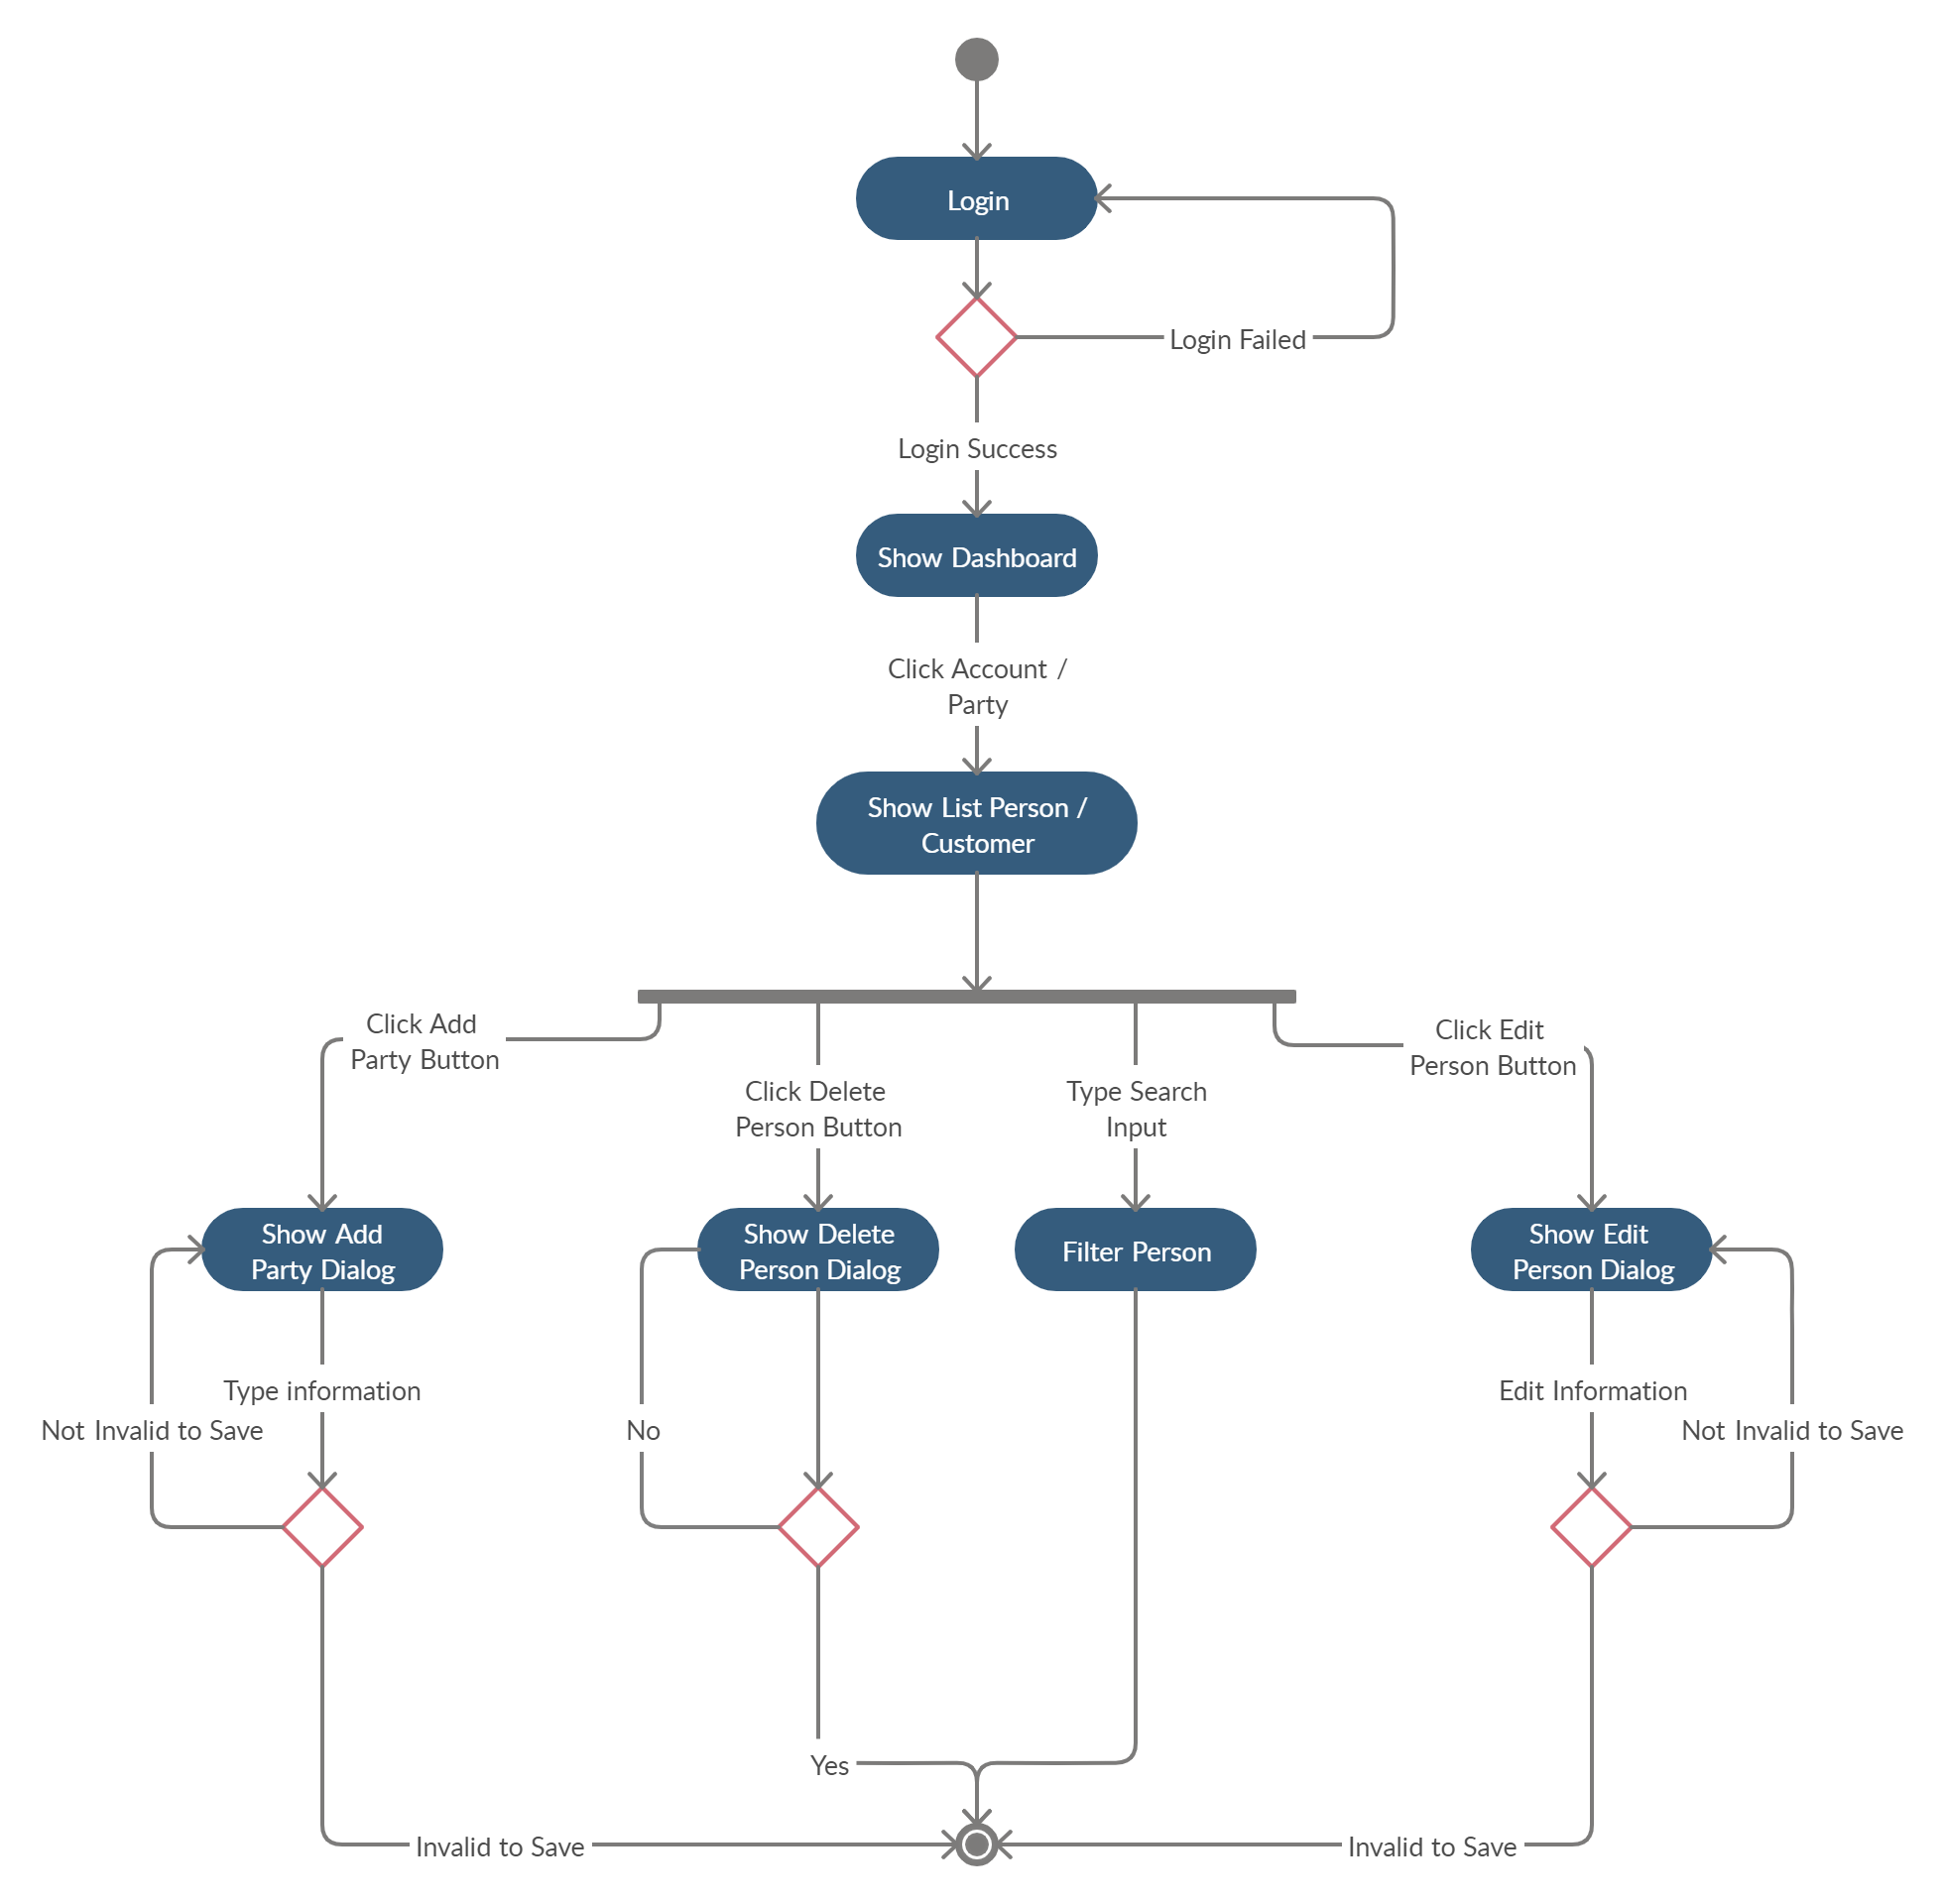
\includegraphics[width=15cm]
{images/activity-diagram/account-management.png}
\caption{Biểu đồ hoạt động ca sử dụng quản lý người dùng}
\end{figure}

Biểu đồ hoạt động cho thao tác phân quyền:
\begin{figure}[H]
\centering
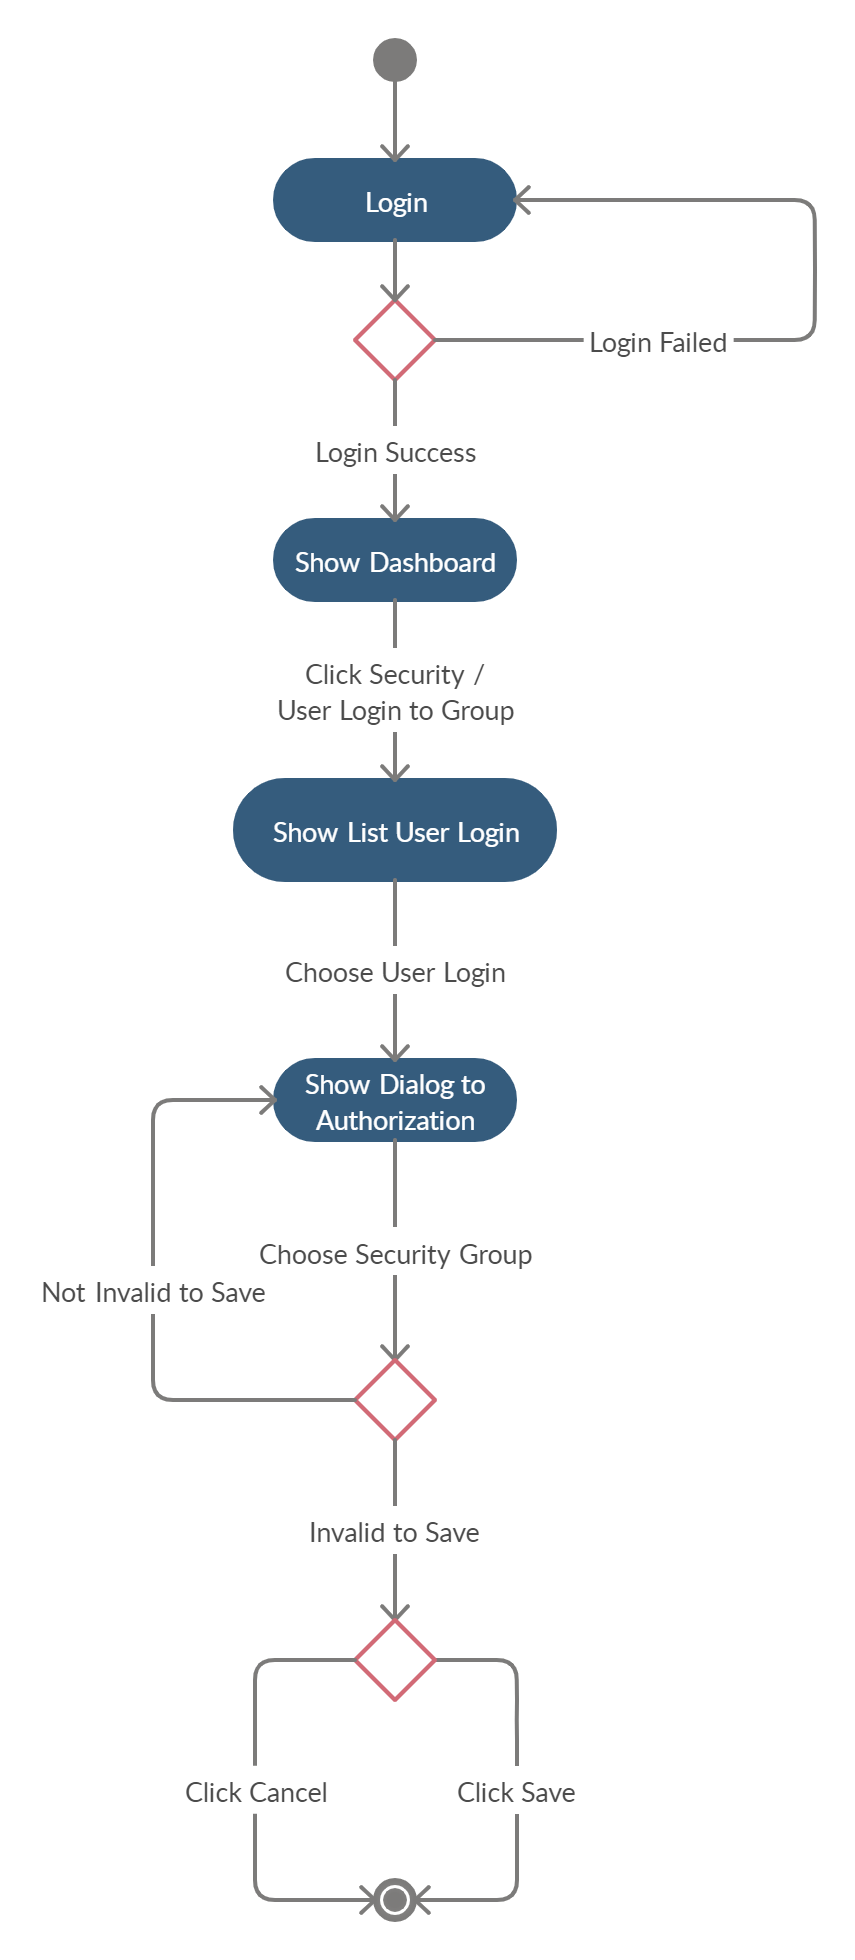
\includegraphics[width=7cm]
{images/activity-diagram/assign-permissions.png}
\caption{Biểu đồ hoạt động cho thao tác phân quyền}
\end{figure}

\subsubsection{Quản lý kho}
Biểu đồ use case cho ca sử dụng quản lý kho:
\begin{figure}[H]
\centering
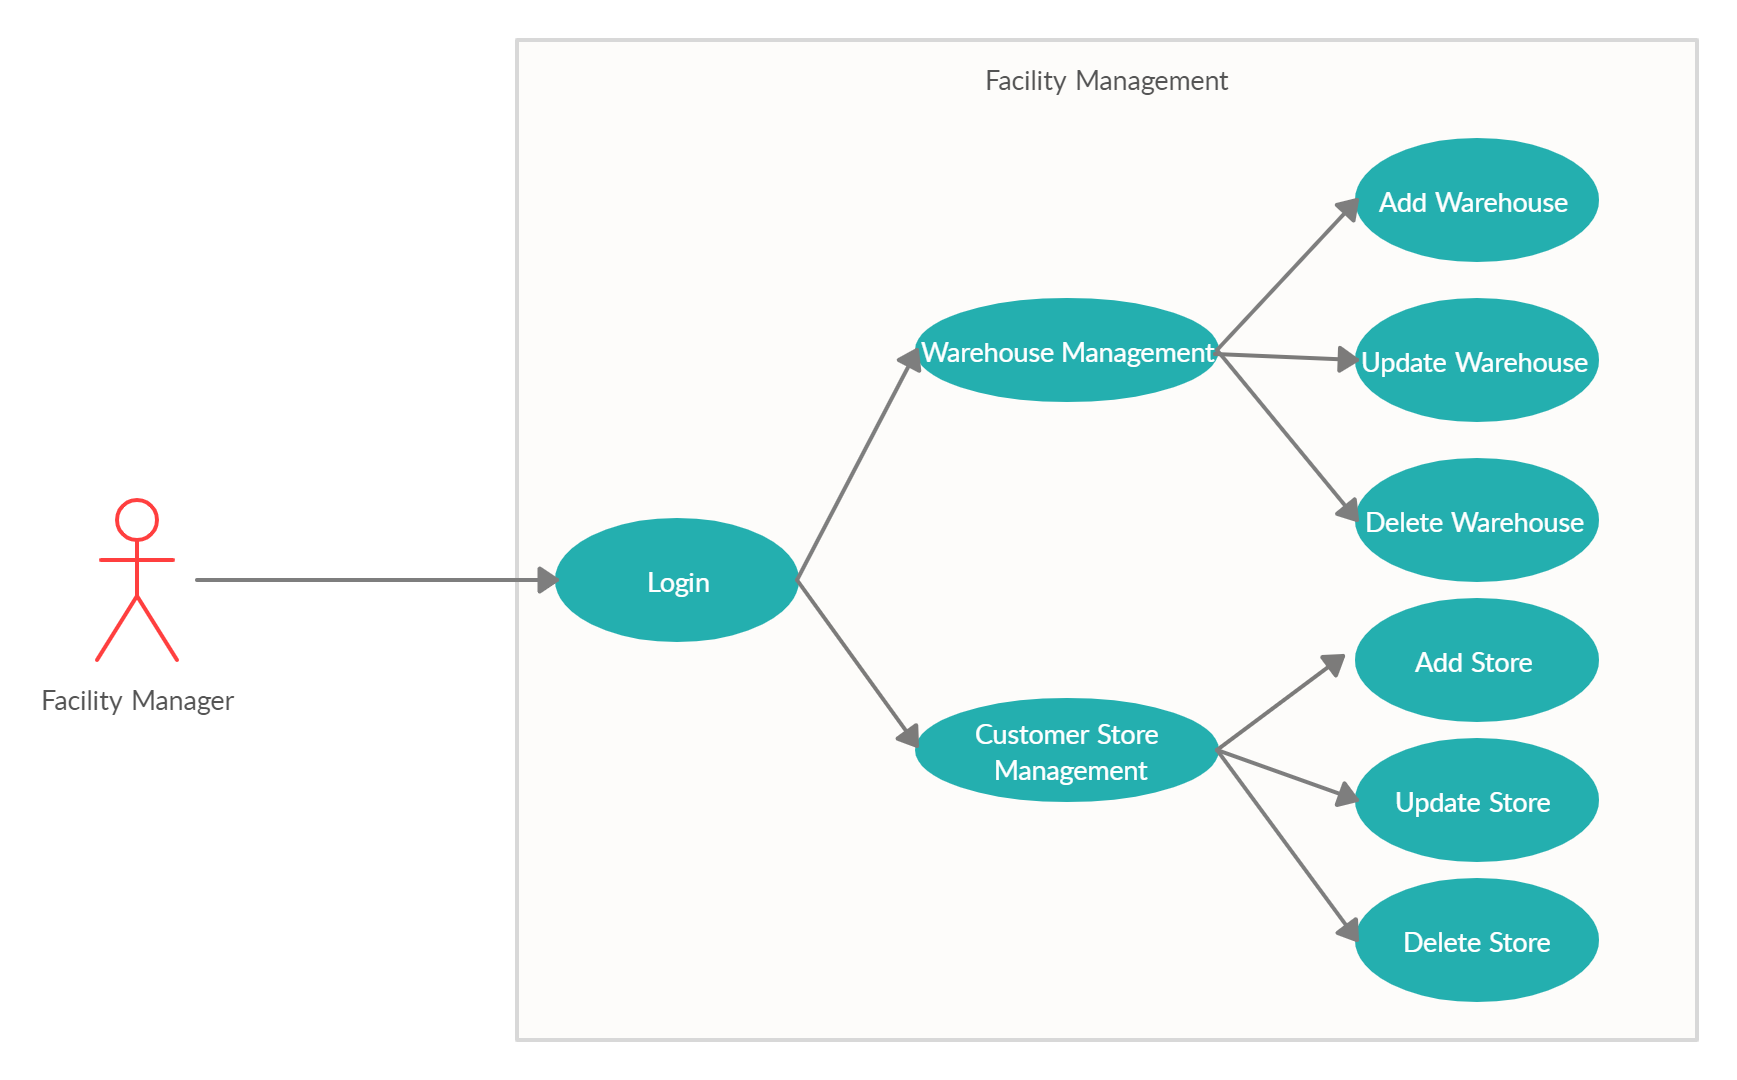
\includegraphics[width=14cm]{images/use-case/facility-management.jpg}
\caption{Use case quản lý kho}
\end{figure}

Người quản lý kho (Facility Manager) nắm được các thông tin
về kho của doanh nghiệp, tập đoàn và kho của cửa hàng bán lẻ,
có thể thêm / sửa / xóa các kho này. 

Biểu đồ hoạt động cho thao tác thêm cửa hàng bán lẻ:
\begin{figure}[H]
\centering
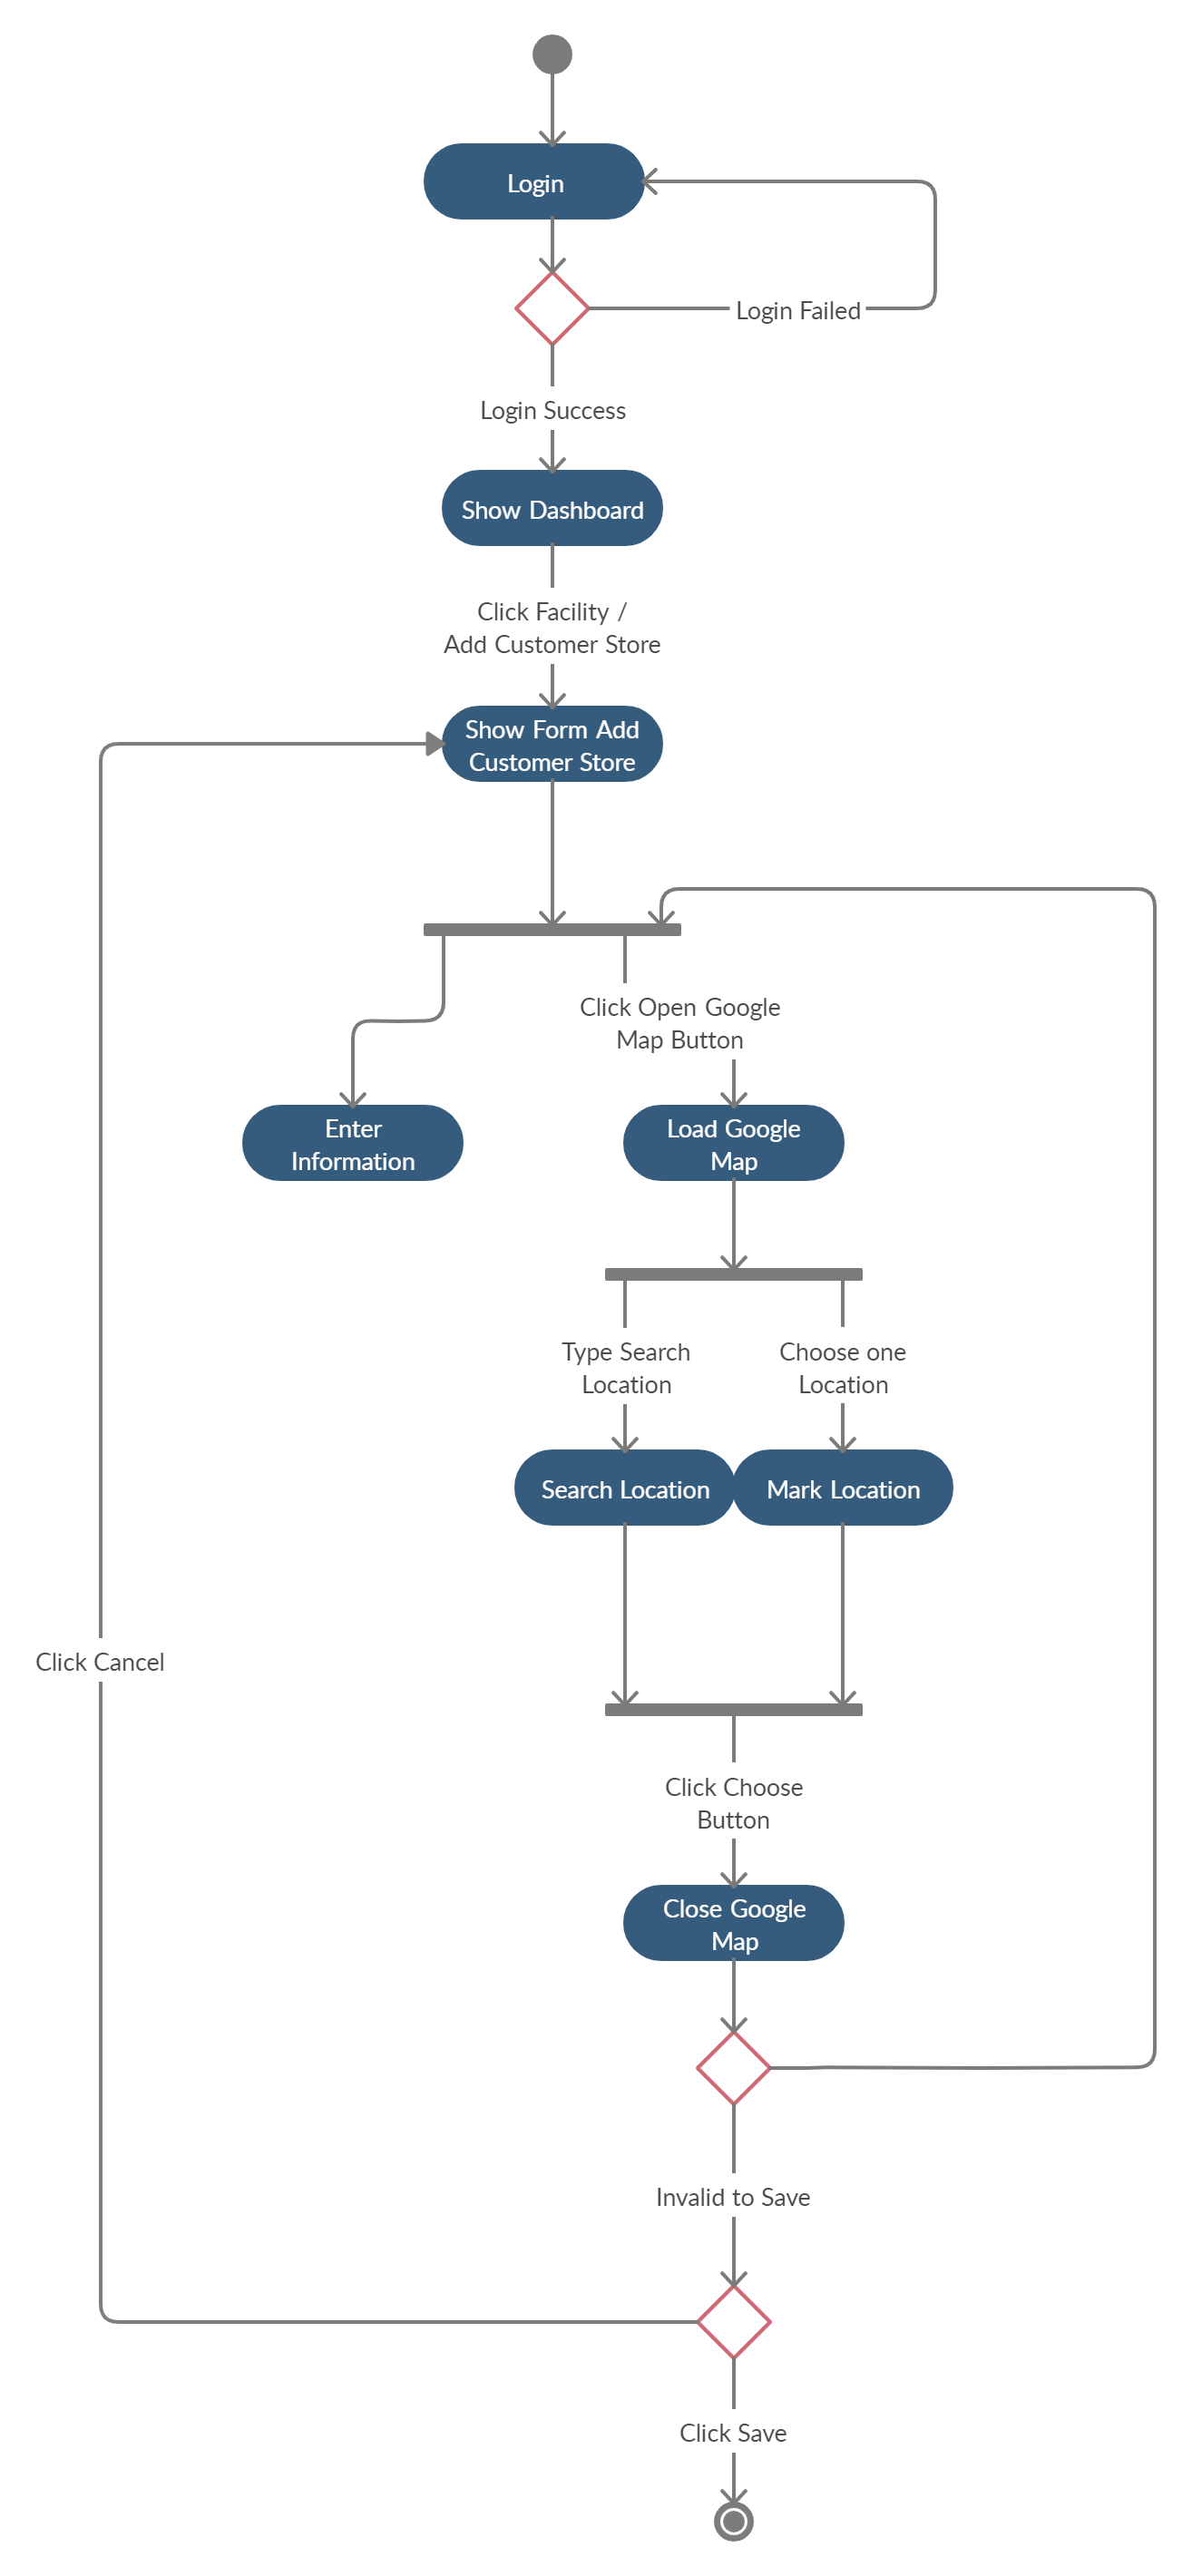
\includegraphics[width=8cm]{images/activity-diagram/add-customer-store.png}
\caption{Biểu đồ hoạt động cho thao tác thêm cửa hàng bán lẻ}
\end{figure}

\subsubsection{Quản lý nhập – xuất hàng}
Biểu đồ use case cho ca sử dụng quản lý nhập – xuất hàng:
\begin{figure}[H]
\centering
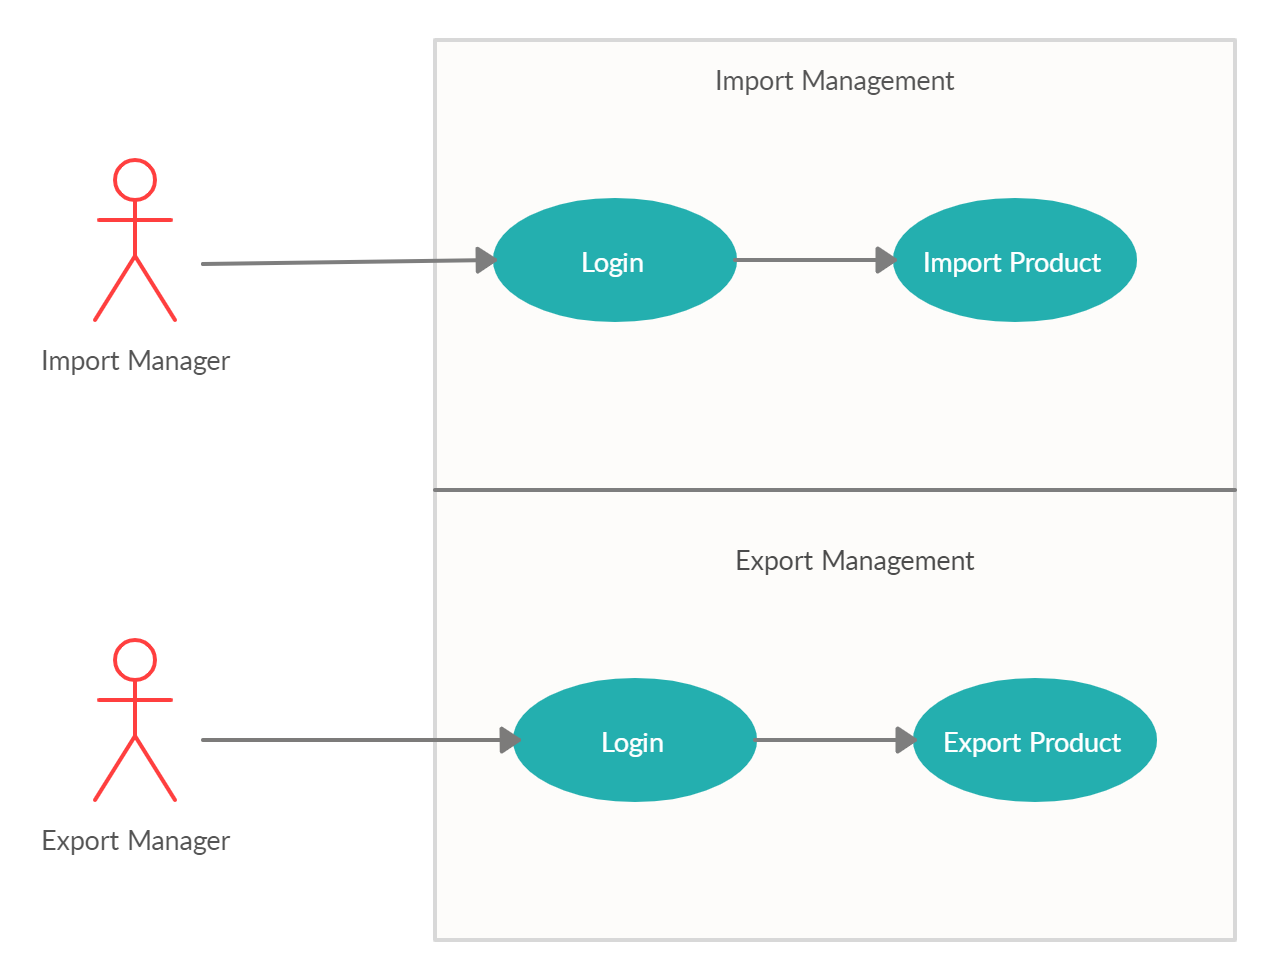
\includegraphics[width=14cm]{images/use-case/import-export.jpg}
\caption{Use case quản lý xuất – nhập hàng}
\end{figure}

Người quản lý nhập hàng (Import Manager) có nhiệm vụ quản lý quy
trình nhập hàng hóa từ nguồn bên ngoài (một doanh nghiệp sản xuất
nào đó hoặc một tập đoàn bán lẻ khác, …) vào kho của doanh nghiệp,
tập đoàn mình. 

Người quản lý xuất hàng (Export Manager) có nhiệm vụ xuất hàng từ
kho của doanh nghiệp, tập đoàn sang các cửa hàng bán lẻ sau khi hóa
đơn xuất hàng đã được duyệt.

\subsubsection{Quản lý sản phẩm}
Biểu đồ use case cho ca sử dụng quản lý sản phẩm:
\begin{figure}[H]
\centering
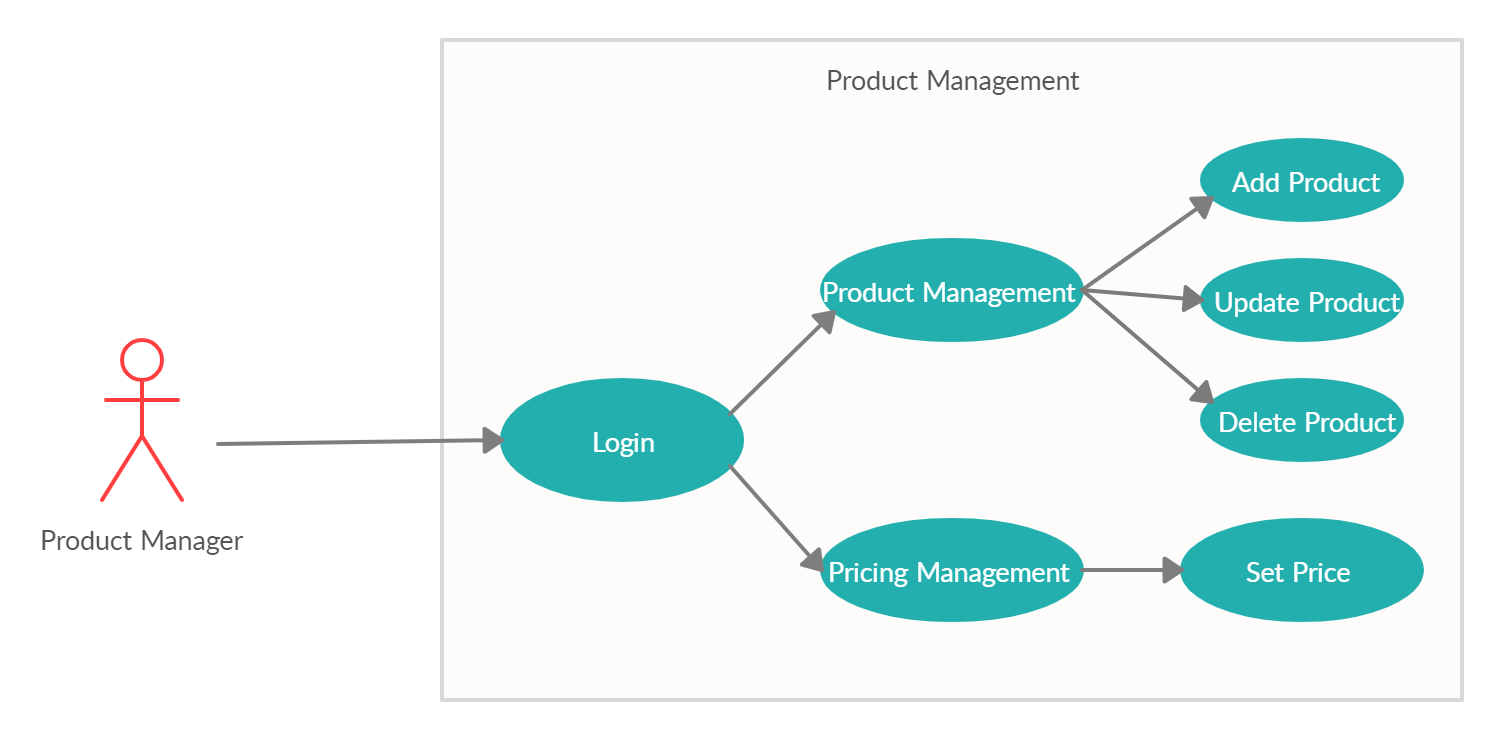
\includegraphics[width=14cm]{images/use-case/product-management.jpg}
\caption{Use-case quản lý sản phẩm}
\end{figure}
Người quản lý sản phẩm (Product Manager) quản lý các sản phẩm
đã được nhập vào và quản lý giá của sản phẩm. 

Biểu đồ hoạt động cho thao tác gán giá cho sản phẩm:
\begin{figure}[H]
\centering
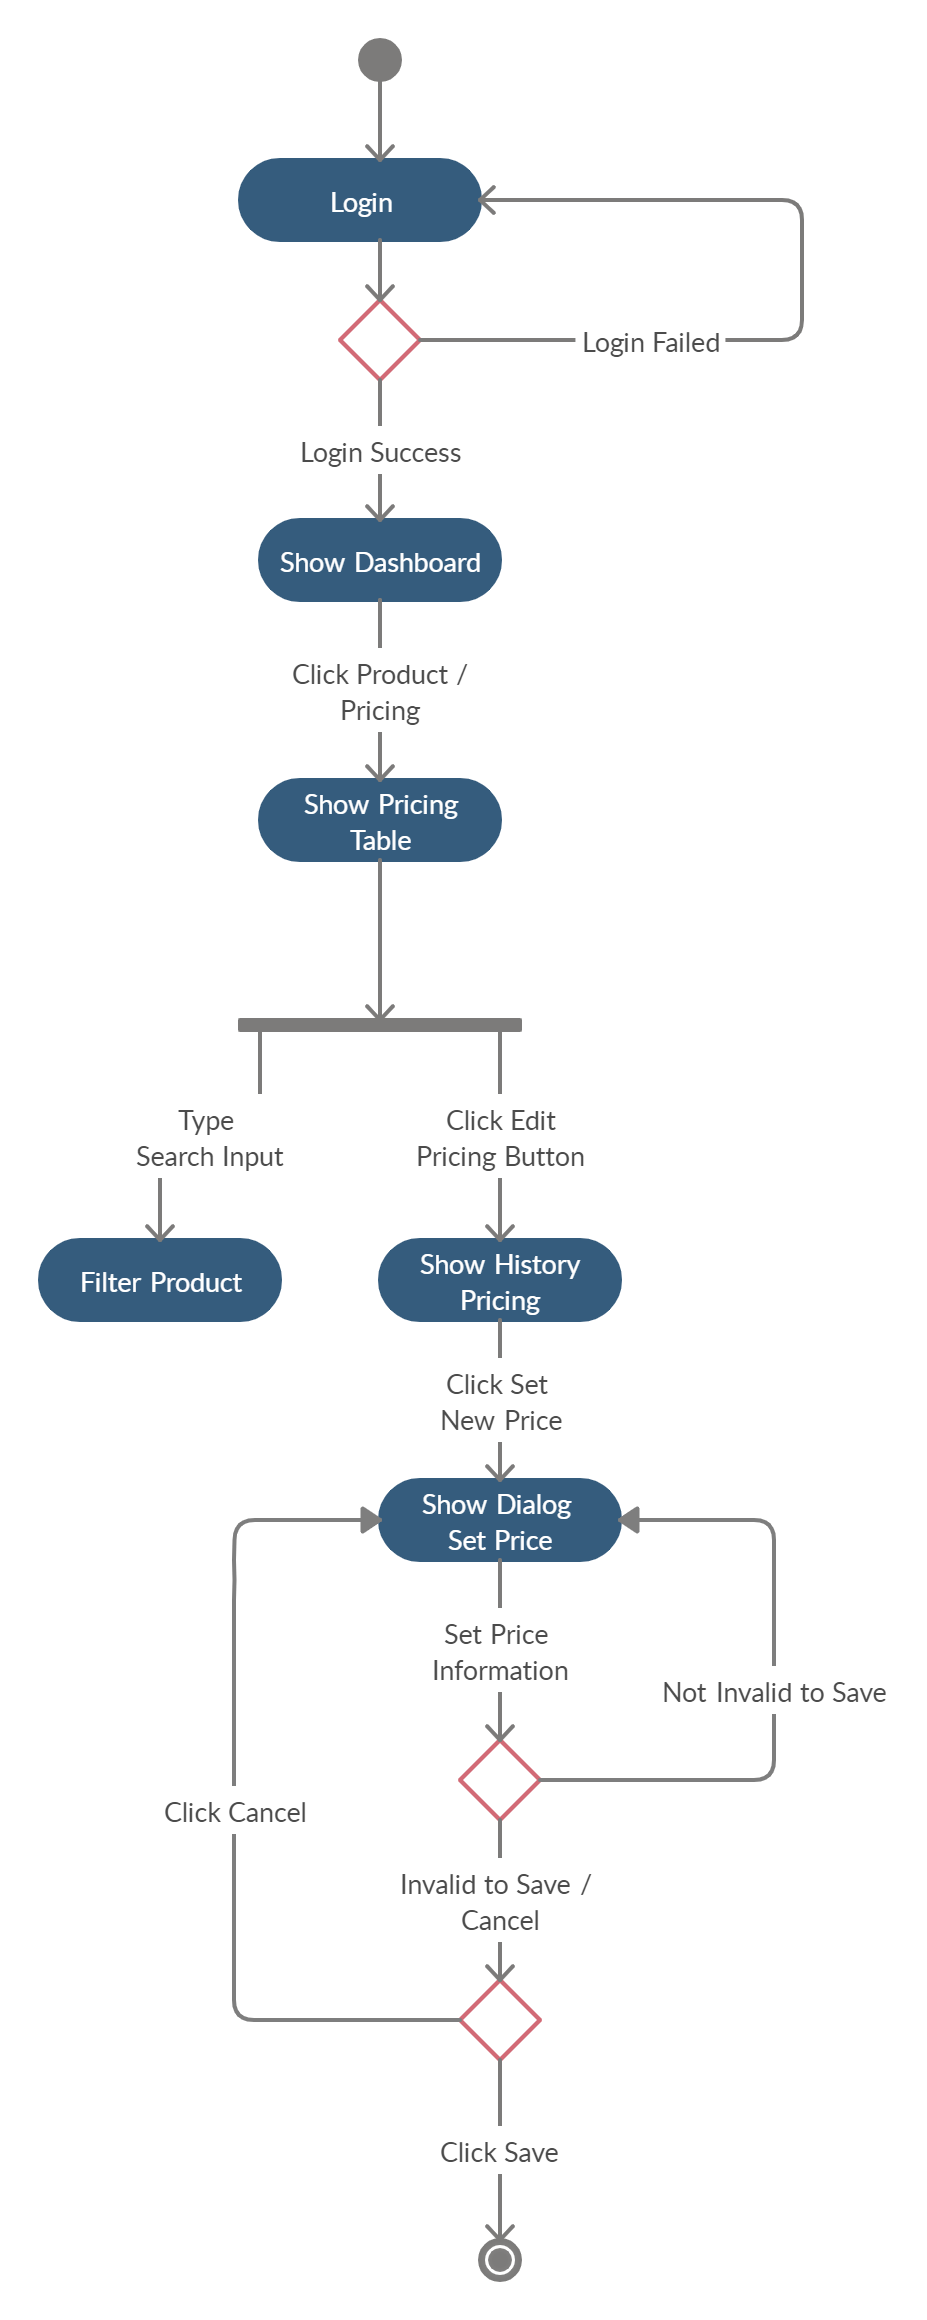
\includegraphics[width=8cm]{images/activity-diagram/set-price.png}
\caption{Biểu đồ hoạt động cho thao tác gán giá của sản phẩm}
\end{figure}

\subsubsection{Quản lý đơn hàng}
Biểu đồ use case cho ca sử dụng quản lý đơn hàng:

(chưa có)

Biểu đồ hoạt động cho thao tác thêm đơn hàng:
\begin{figure}[H]
\centering
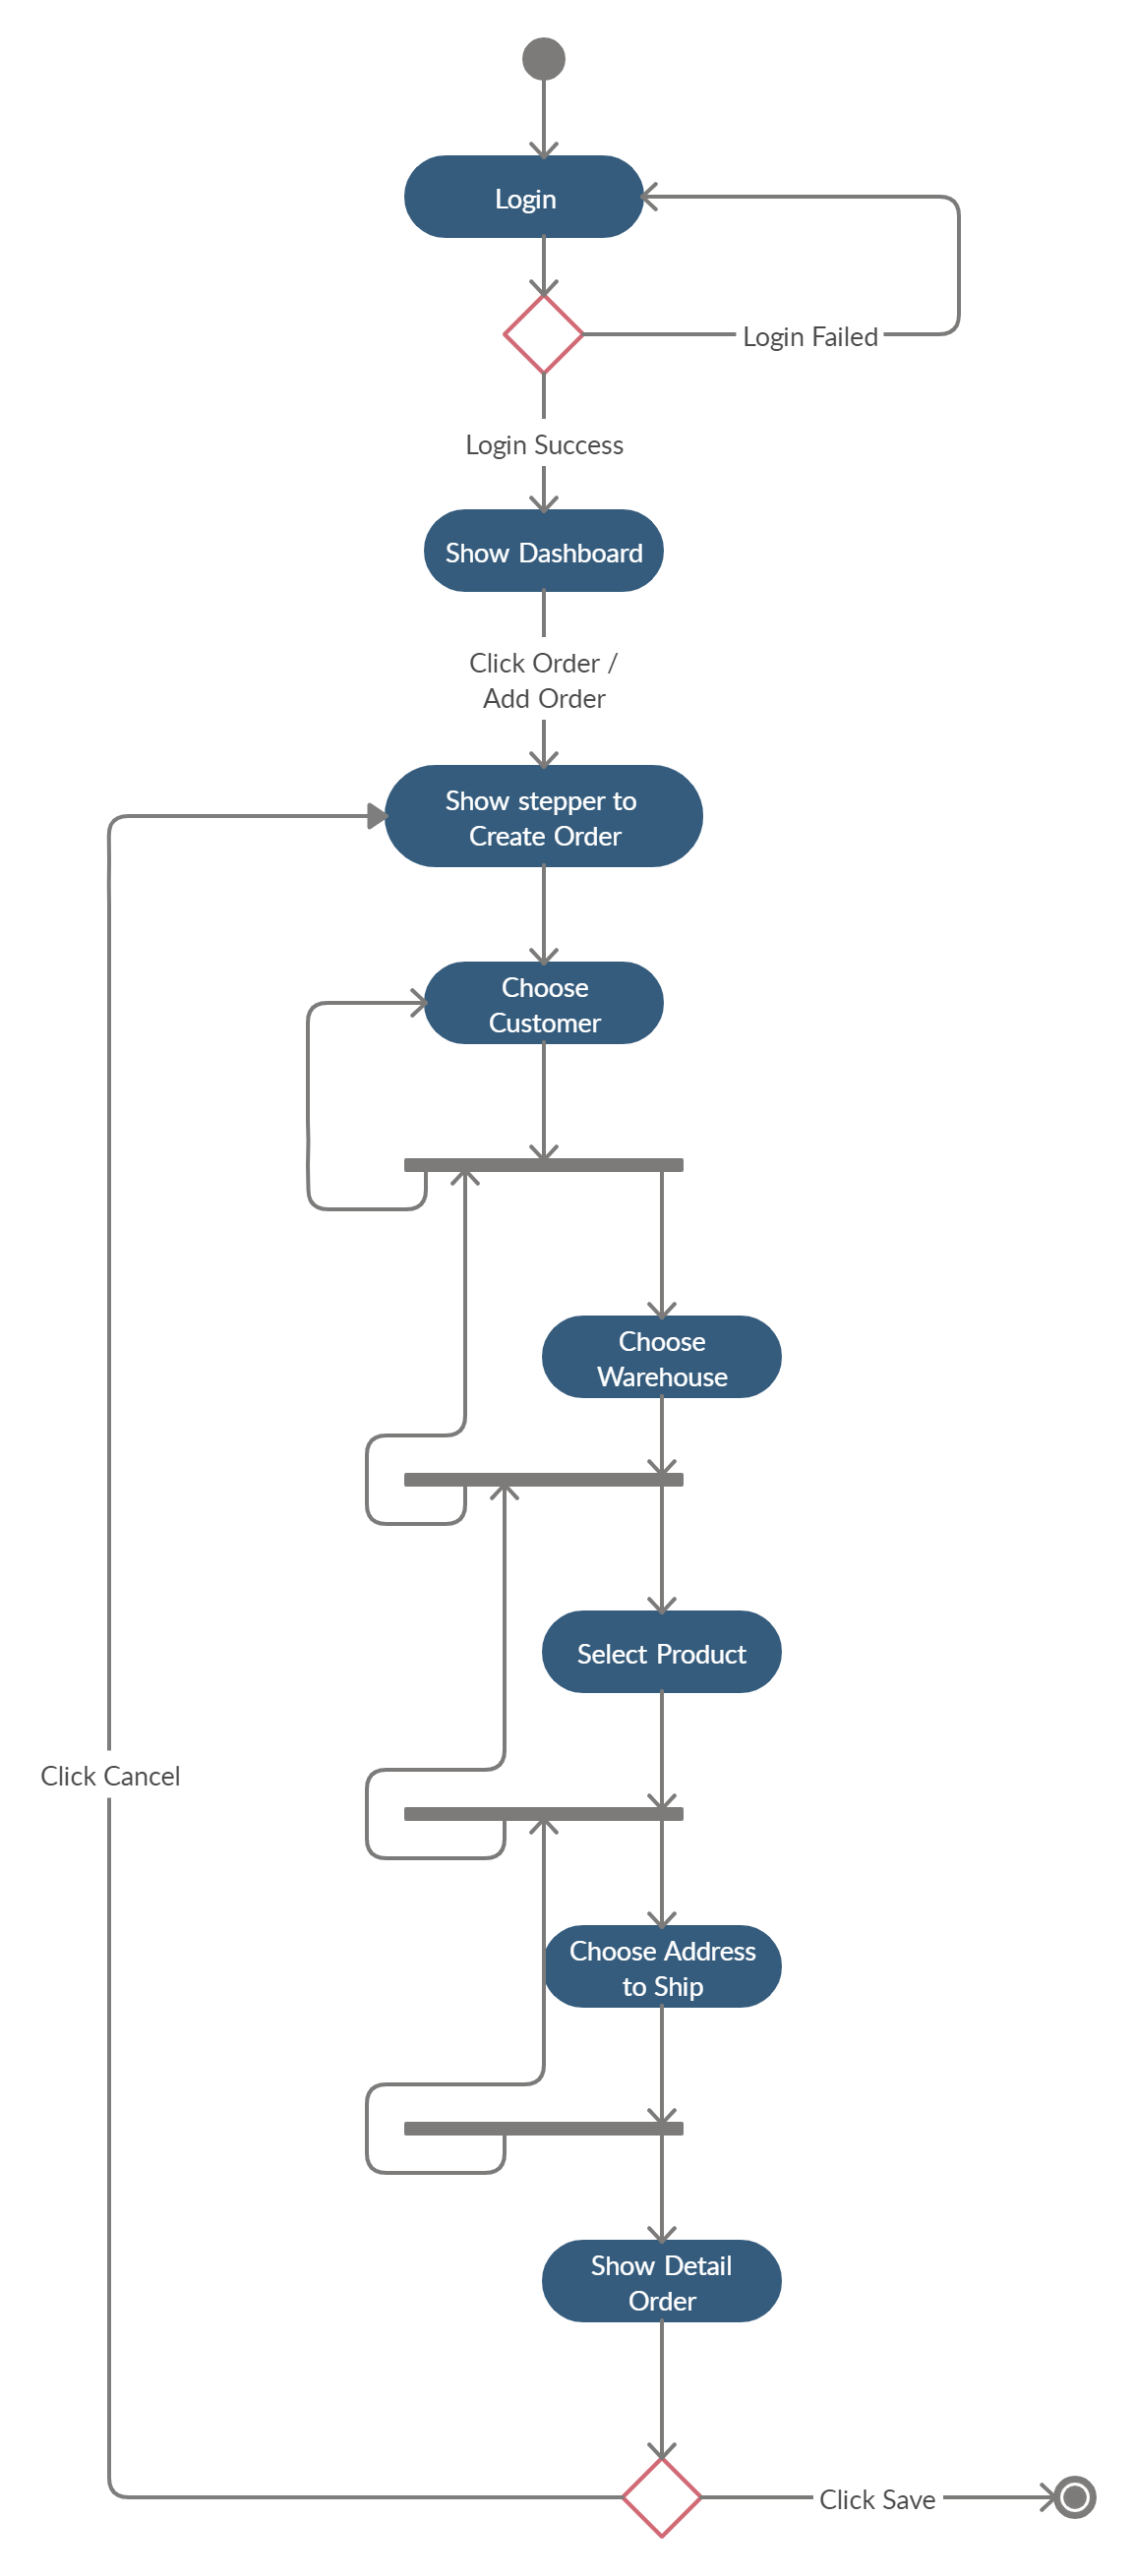
\includegraphics[width=8cm]{images/activity-diagram/add-order.png}
\caption{Biểu đồ hoạt động cho thao tác thêm đơn hàng}
\end{figure}

\subsubsection{Quản lý tuyến bán hàng}
Biểu đồ use case cho ca sử dụng quản lý tuyến bán hàng:
\begin{figure}[H]
\centering
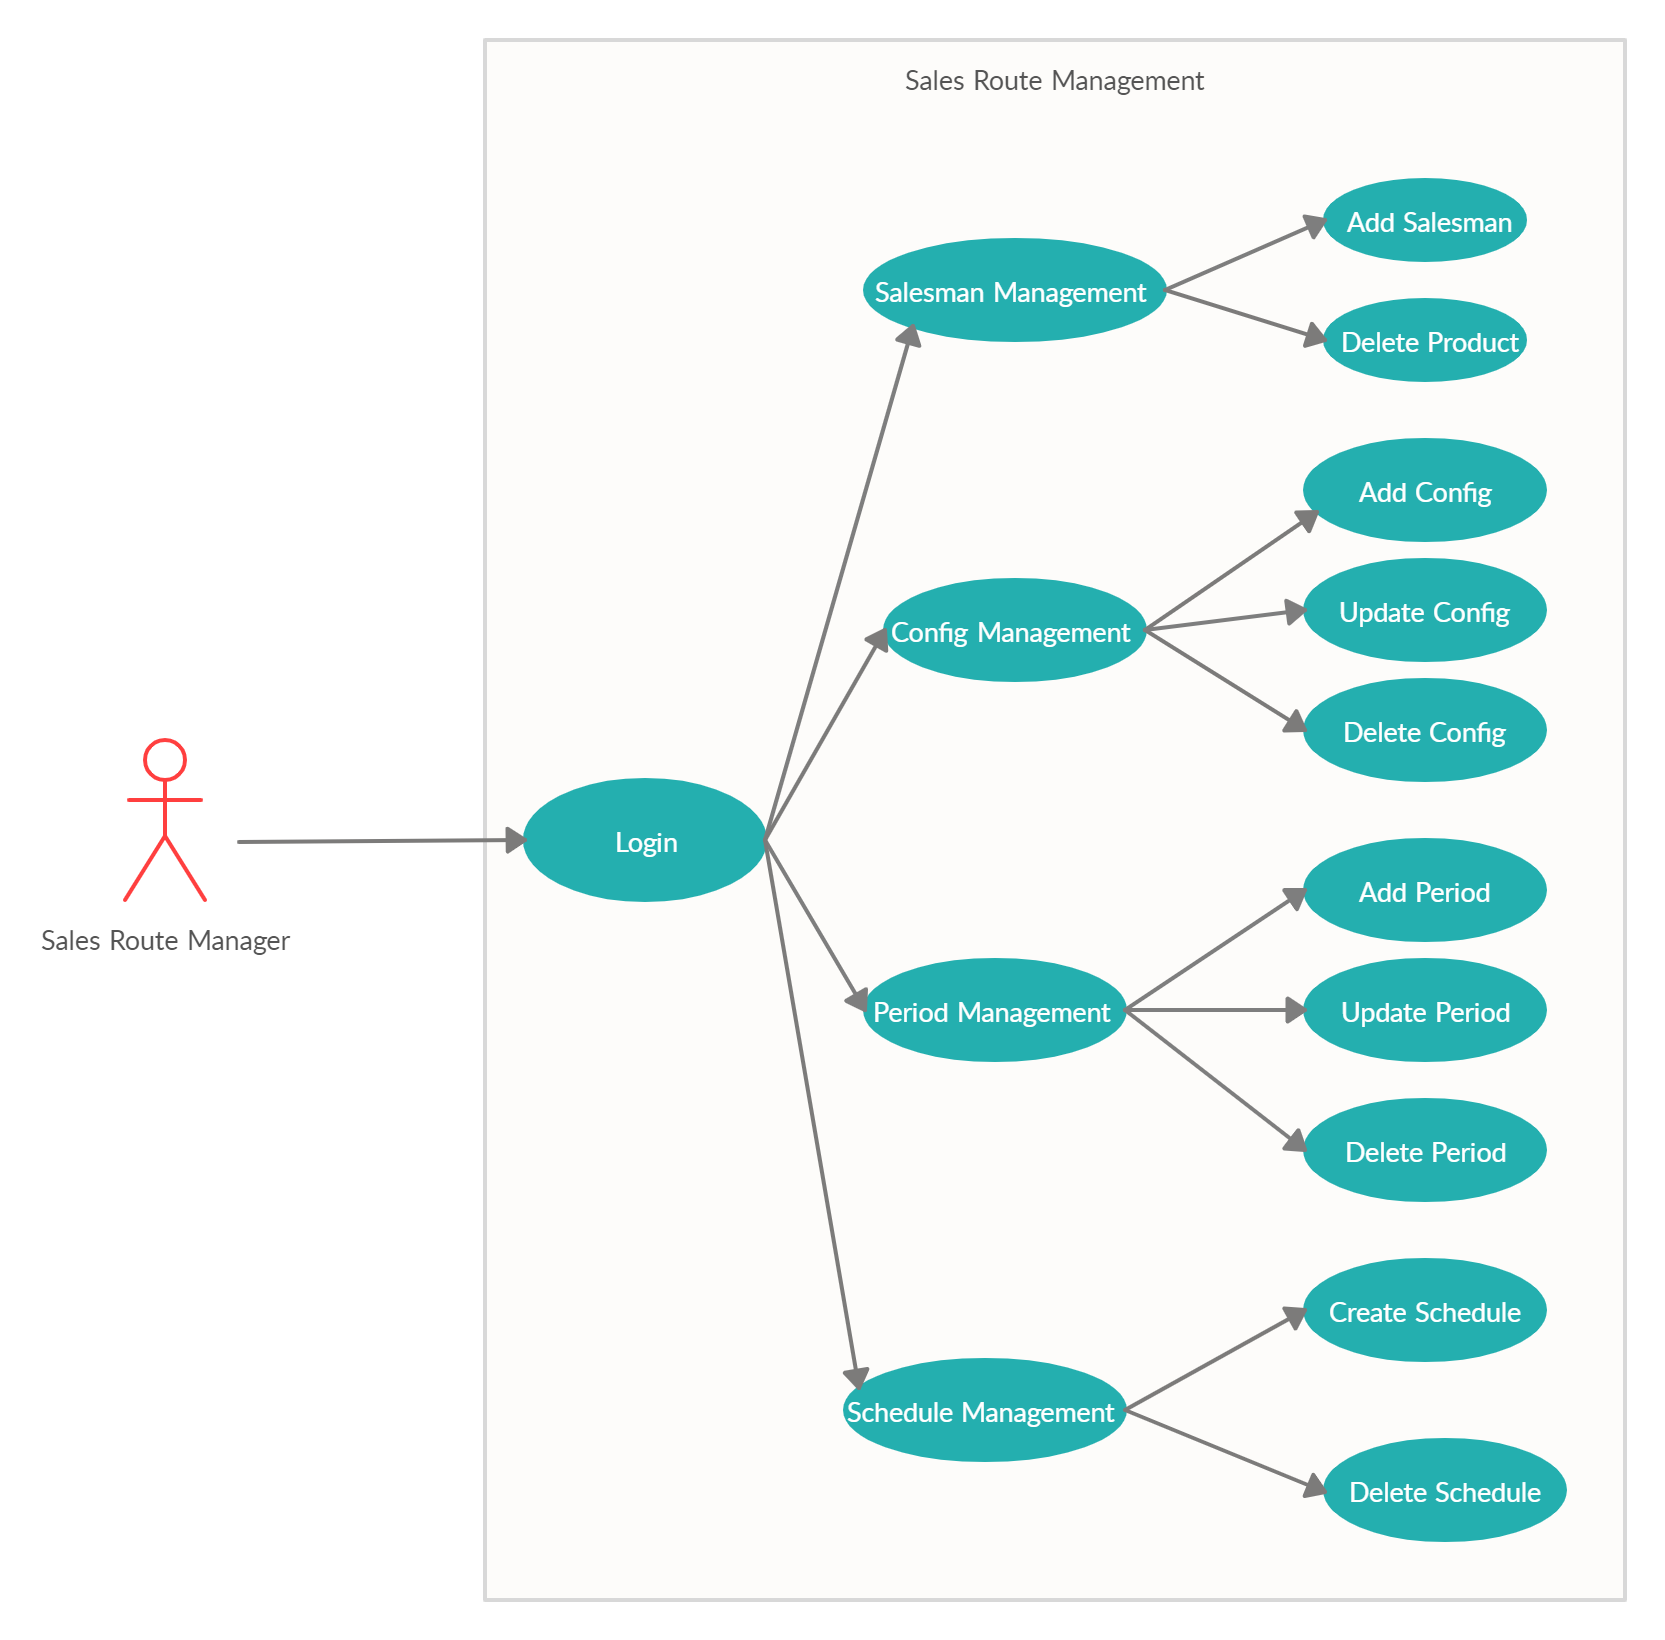
\includegraphics[width=14cm]{images/use-case/sales-route.png}
\caption{Use case quản lý tuyến bán hàng}
\end{figure}
Người quản lý tuyến bán hàng (Sales Route Manager) quản lý danh
sách tuyến, cấu hình các tuyến, lên lịch trình tuyến cho
nhân viên bán hàng.

Biểu đồ hoạt động cho thao tác thêm tuyến bán
hàng cho nhân viên bán hàng:
\begin{figure}[H]
\centering
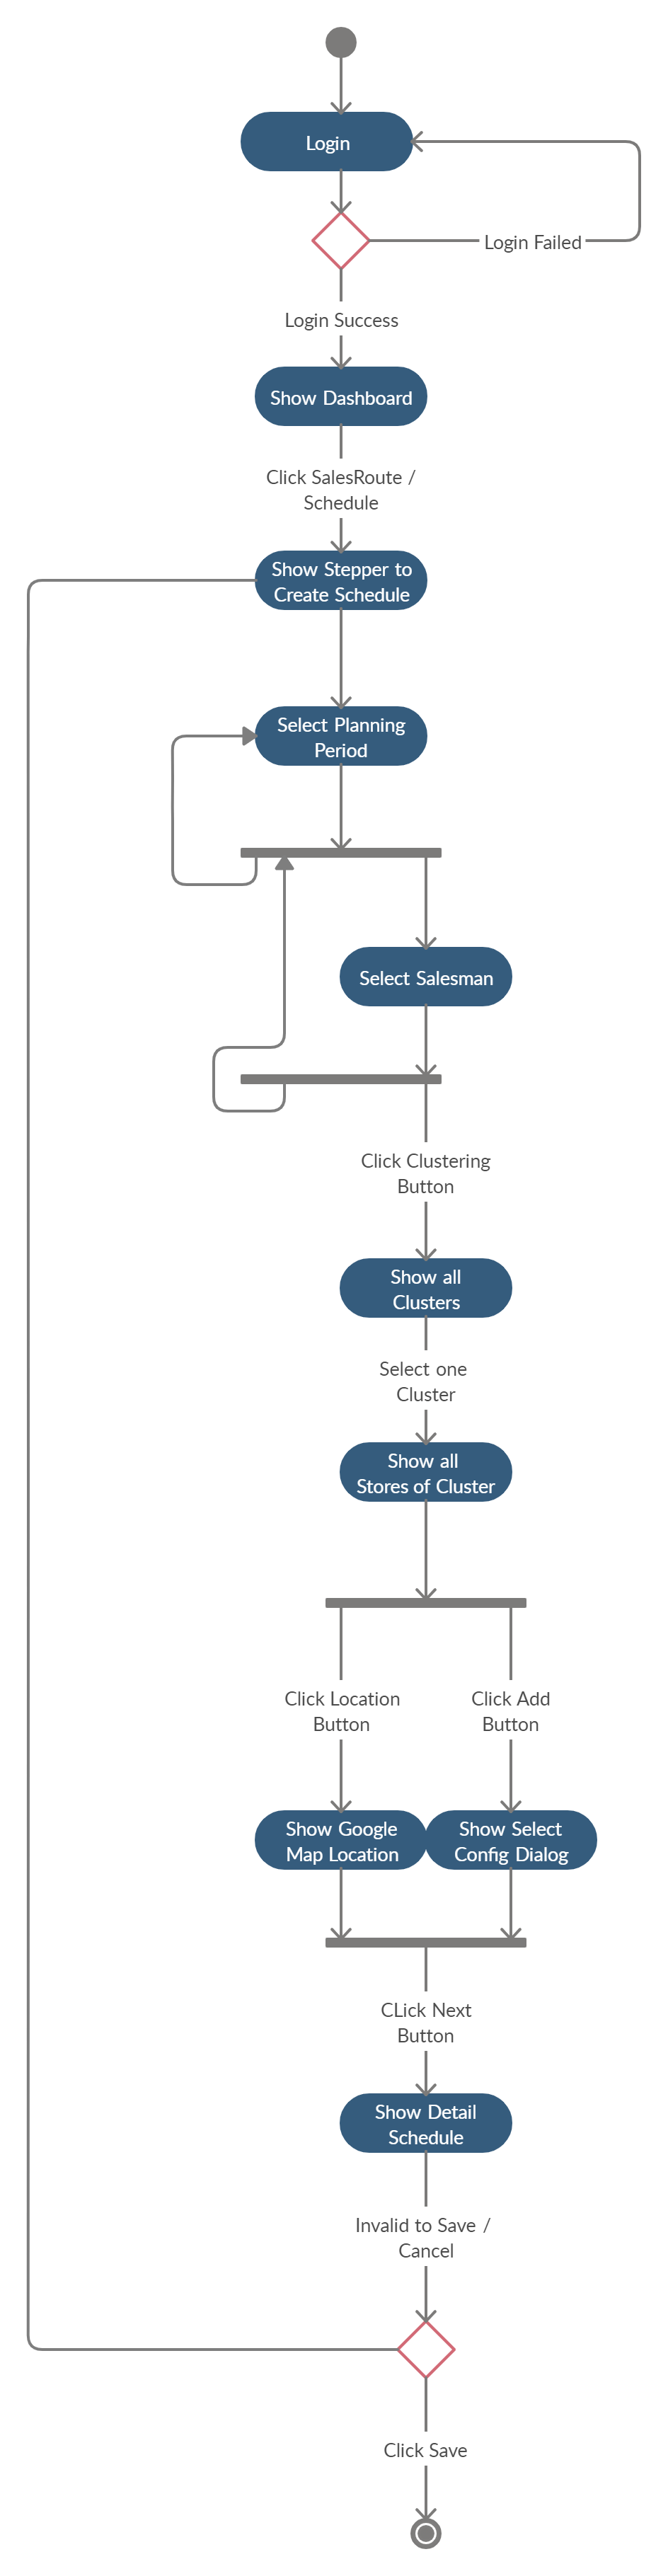
\includegraphics[width=6cm]{images/activity-diagram/add-schedule.png}
\caption{Biểu đồ hoạt động cho thao tác thêm tuyến bán hàng cho
nhân viên bán hàng}
\end{figure}

\subsubsection{Nhân viên bán hàng check-in}
Biểu đồ use case cho ca sử dụng nhân viên bán hàng check-in:
\begin{figure}[H]
\centering
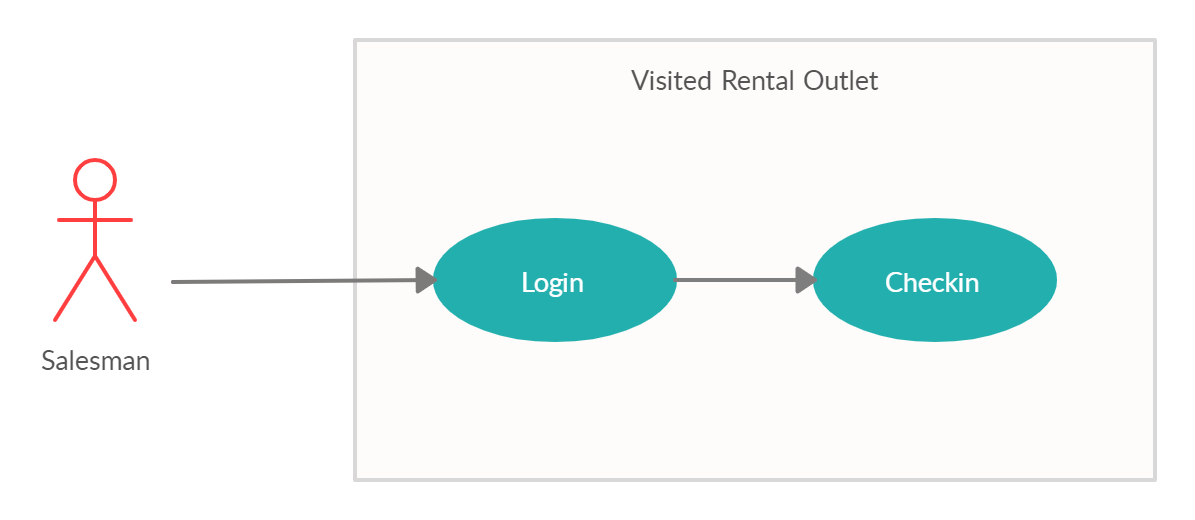
\includegraphics[width=14cm]{images/use-case/salesman.jpg}
\caption{Use-case nhân viên bán hàng check-in}
\end{figure}
Khi nhân viên bán hàng đến check-in tại cửa hàng bán lẻ,
hệ thống sẽ lưu lại thông tin về vị trí, thời điểm nhân
viên bán hàng check-in.

\section{Thiết kế cơ sở dữ liệu}
Phần này trình bày chi tiết thiết kế các bảng của cơ sở dữ
liệu sử dụng PostgreSQL phục vụ cho việc triển khai các use case
đã trình bày ở trên.

Nhóm các bảng phục vụ chức năng quản lý phân quyền, quản lý
người dùng được trình bày qua sơ đồ thực thể liên kết
(Hình~\ref{fig:dbsecurity}) và bảng thông tin (Bảng~\ref{tab:dbsecurity}).

\begin{figure}[H]
\centering
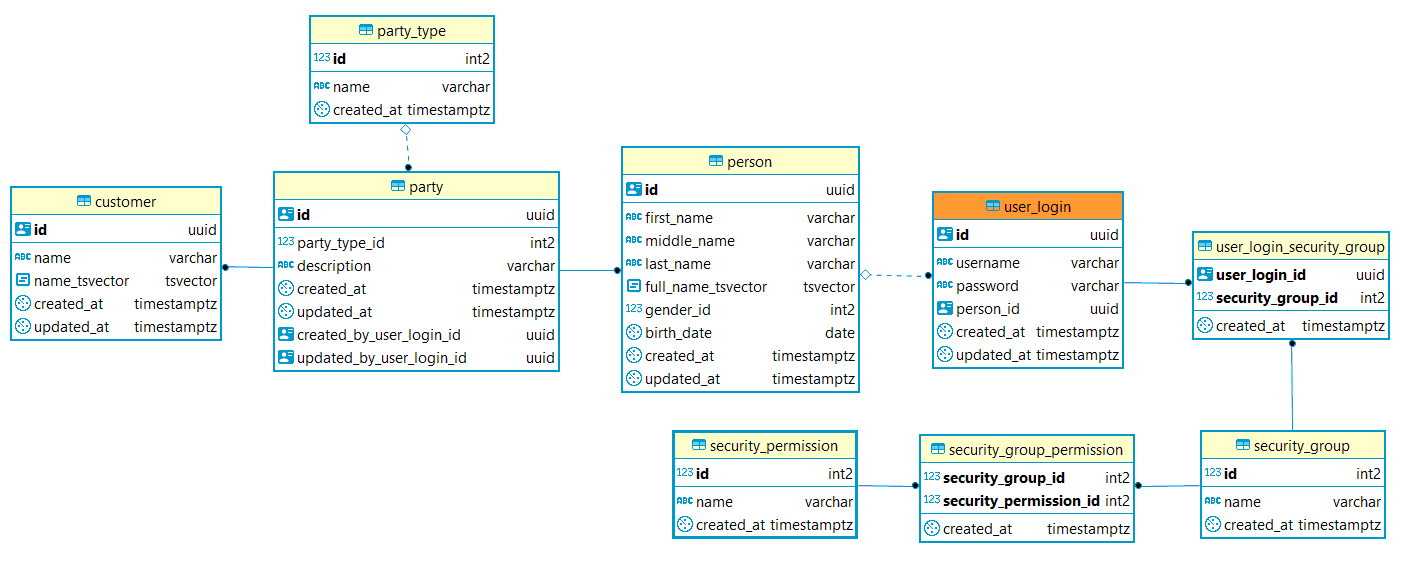
\includegraphics[width=17cm]{images/database/security.png}
\caption{Cơ sở dữ liệu quản lý phân quyền, người dùng}
\label{fig:dbsecurity}
\end{figure}

\begin{table}[H]
\centering
\begin{tabular}{| m{5cm} | m{10cm} |}
\hline
\textbf{Tên bảng} & \textbf{Thông tin chính được thể hiện} \\
\hline
party\_type & Loại người dùng (nhân viên, khách hàng) \\
\hline
party & Danh sách thông tin người dùng \\
\hline
customer & Danh sách thông tin khách hàng \\
\hline 
person & Danh sách thông tin một nhân viên \\
\hline 
user\_login & Danh sách thông tin một tài khoản \\
\hline 
security\_group &
Danh sách các role (account manager, product manager, …) \\
\hline
security\_permission &
Danh sách các quyền (ADD\_USER, EDIT\_SALESMAN, …) \\
\hline
\end{tabular}
\caption{Thông tin các bảng nhóm quản lý phân quyền, người dùng}
\label{tab:dbsecurity}
\end{table}

Nhóm các bảng phục vụ chức năng quản lý đơn hàng được
trình bày qua sơ đồ thực thể liên kết (Hình~\ref{fig:dborder})
và bảng thông tin (Bảng~\ref{tab:dborder}).
\begin{figure}[H]
\centering
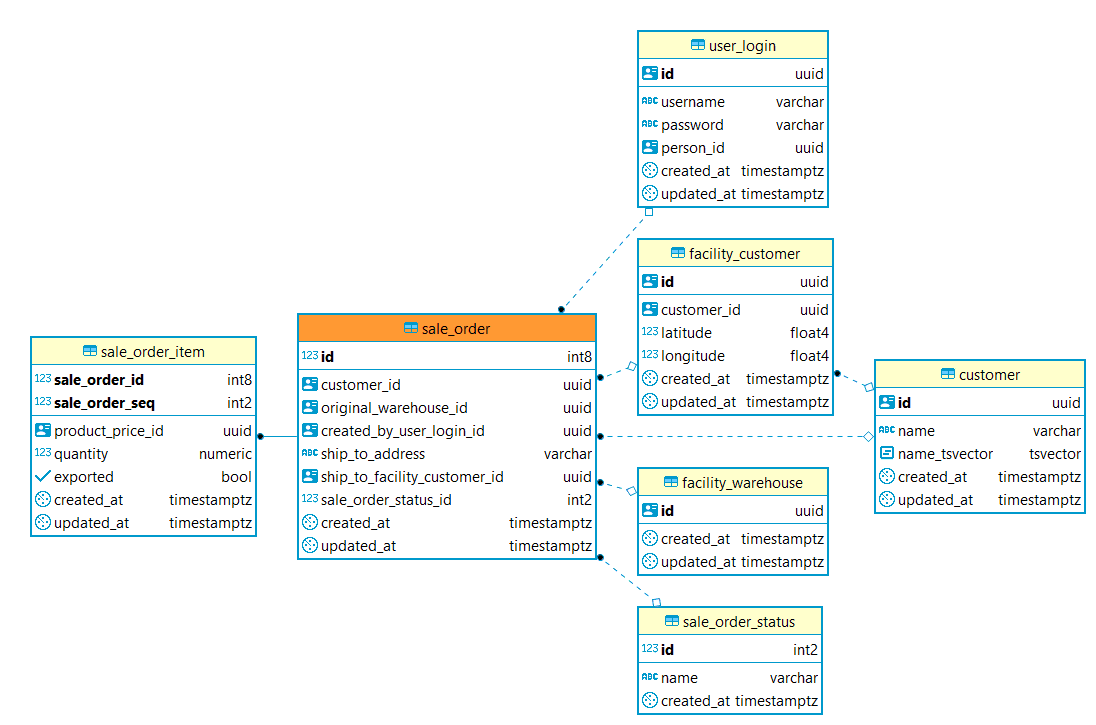
\includegraphics[width=17cm]{images/database/order.png}
\caption{Cơ sở dữ liệu quản lý đơn hàng}
\label{fig:dborder}
\end{figure}

\begin{table}[H]
\centering
\begin{tabular}{| m{5cm} | m{10cm} |}
\hline
\textbf{Tên bảng} & \textbf{Thông tin chính được thể hiện} \\
\hline
sale\_order &
Danh sách thông tin đơn hàng \\
\hline
sale\_order\_item &
Danh sách các item trong đơn hàng \\
\hline
facility\_customer &
Danh sách thông tin cửa hàng bán lẻ \\
\hline
facility\_warehouse &
Danh sách thông tin kho  \\
\hline
sale\_order\_status &
Trạng thái của đơn hàng \\
\hline
\end{tabular}
\caption{Thông tin các bảng nhóm quản lý phân quyền, người dùng}
\label{tab:dborder}
\end{table}

Nhóm các bảng phục vụ chức năng quản lý sản phẩm
được trình bày qua sơ đồ thực thể liên kết (Hình~\ref{fig:dbproduct})
và bảng thông tin (Bảng~\ref{tab:dbproduct}).
\begin{figure}[H]
\centering
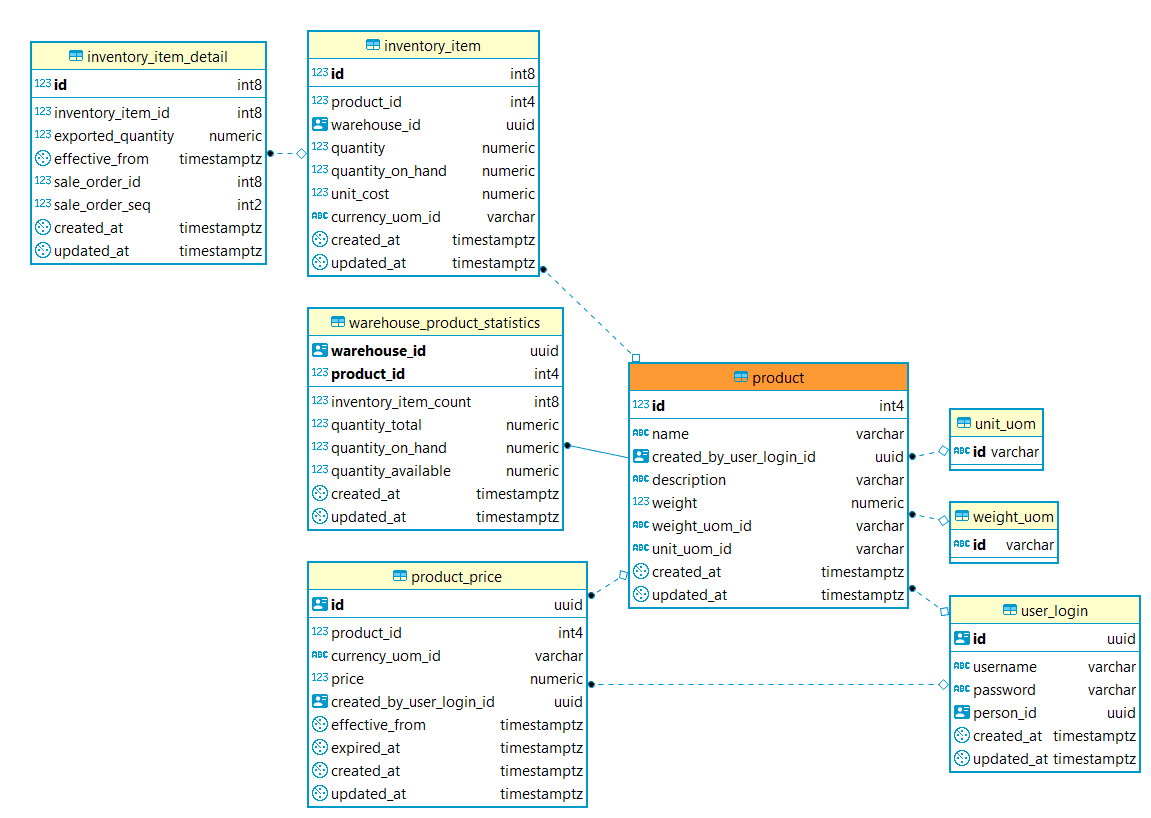
\includegraphics[width=17cm]{images/database/product.png}
\caption{Cơ sở dữ liệu quản lý đơn hàng}
\label{fig:dbproduct}
\end{figure}

\begin{table}[H]
\centering
\begin{tabular}{| m{6cm} | m{10cm} |}
\hline
\textbf{Tên bảng} & \textbf{Thông tin chính được thể hiện} \\
\hline

product &
Danh sách thông tin sản phẩm (product nói chung, chưa nhập kho) \\
\hline
product\_price &
Thông tin giá ứng với sản phẩm \\
\hline
warehouse\_product\_statistics &
Thống kê các thông tin của sản phẩm
(số lượng tổng, số lượng đặt, số lượng có sẵn, …) \\
\hline
inventory\_item &
Thông tin sản phẩm trong kho  \\
\hline
inventory\_item\_detail &
Thông tin chi tiết đối với từng sản phẩm trong kho \\
\hline
unit\_uom &
Đơn vị hình dạng (hộp, chai, gói) \\
\hline
weight\_uom &
Đơn vị khối lượng (kg, g, mg) \\

\hline
\end{tabular}
\caption{Thông tin các bảng nhóm quản lý sản phẩm}
\label{tab:dbproduct}
\end{table}

Nhóm các bảng phục vụ chức năng quản lý tuyến bán hàng
được trình bày qua sơ đồ thực thể liên kết (Hình~\ref{fig:dbsalesroute})
và bảng thông tin (Bảng~\ref{tab:dbsalesroute}).
\begin{figure}[H]
\centering
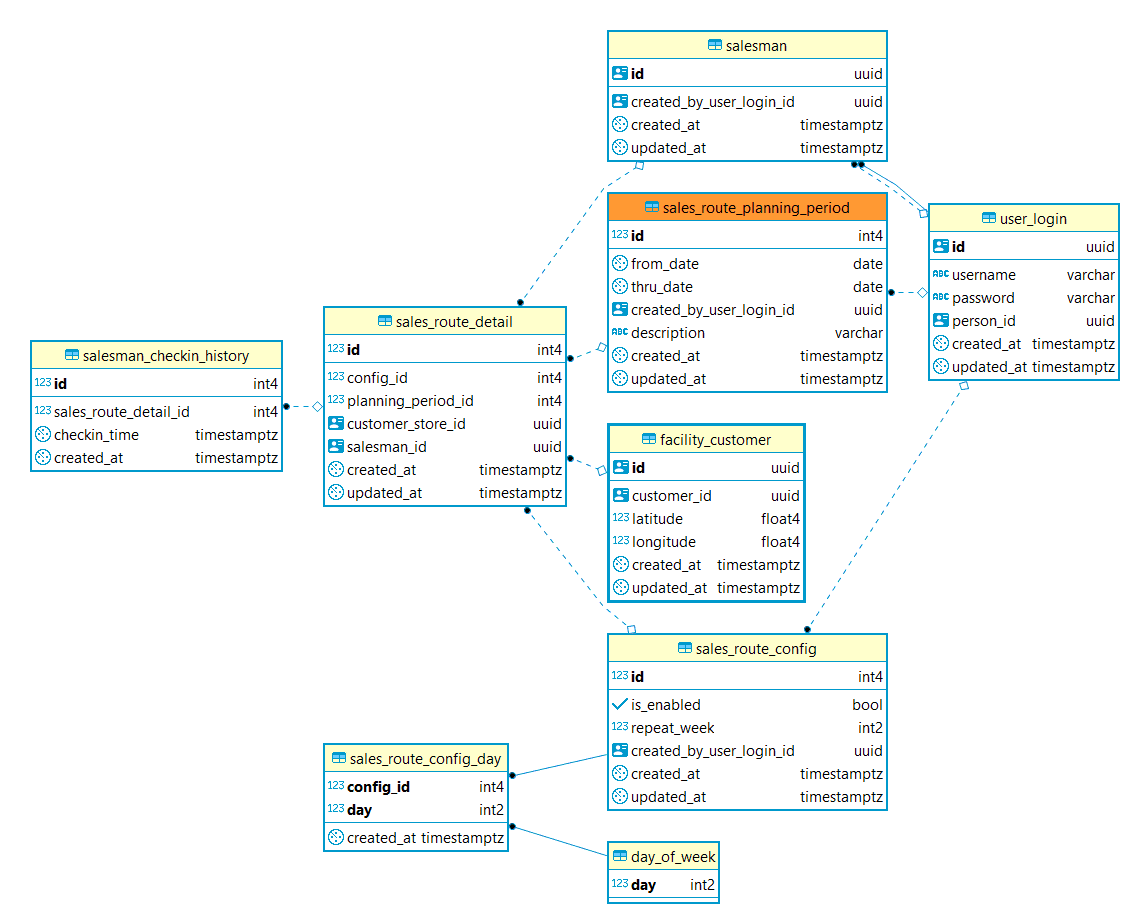
\includegraphics[width=17cm]{images/database/sales-route.png}
\caption{Cơ sở dữ liệu quản lý tuyến bán hàng}
\label{fig:dbsalesroute}
\end{figure}

\begin{table}[H]
\centering
\begin{tabular}{| m{6cm} | m{10cm} |}
\hline
\textbf{Tên bảng} & \textbf{Thông tin chính được thể hiện} \\
\hline
salesman &
Danh sách thông tin nhân viên bán hàng \\
\hline
sales\_route\_planning\_period &
Danh sách thông tin tuyến bán hàng
(thời gian bắt đầu – thời gian kết thúc) \\
\hline
sales\_route\_config &
Danh sách thông tin cấu hình tuyến bán hàng
(thăm cửa hàng vào thứ nào, mấy tuần một lần) \\
\hline
sales\_route\_detail &
Chi tiết tuyến bán hàng \\
\hline
salesman\_checkin\_history &
Thông tin checkin của nhân viên bán hàng  \\
\hline
day\_of\_week &
Danh sách các ngày trong tuần \\
\hline
\end{tabular}
\caption{Thông tin các bảng nhóm quản lý tuyến bán hàng}
\label{tab:dbsalesroute}
\end{table}
